%-------------------------------------------------------------------------------
%                      Template Naskah Skripsi
%               	Berdasarkan format JTETI FT UGM
% 						(c) @gunturdputra 2014
%-------------------------------------------------------------------------------

%Template pembuatan naskah skripsi.
\documentclass{mipathesis}

%Untuk prefiks pada daftar gambar dan tabel
\usepackage[titles]{tocloft}
\renewcommand\cftfigpresnum{Gambar\  }
\renewcommand\cfttabpresnum{Tabel\   }

%Untuk hyperlink dan table of content
\usepackage{hyperref}
\newlength{\mylenf}
\settowidth{\mylenf}{\cftfigpresnum}
\setlength{\cftfignumwidth}{\dimexpr\mylenf+2em}
\setlength{\cfttabnumwidth}{\dimexpr\mylenf+2em}

%Untuk Bold Face pada Keterangan Gambar
\usepackage[labelfont=bf]{caption}

%Untuk caption dan subcaption
\usepackage{caption}
\usepackage{subcaption}


%-----------------------------------------------------------------
%Disini awal masukan untuk data proposal skripsi
%-----------------------------------------------------------------
\titleind{PENCARIAN INFORMASI FASILITAS UMUM KOTA PALEMBANG BERBASIS SEMANTIK WEB MENGGUNAKAN QUERY BAHASA ALAMI}

\fullname{Rijalul Fikri}

\idnum{13/356469/PPA/04468}

\approvaldate{1 Juli 2017}

\degree{Master Computer Science}

\yearsubmit{2017}

\program{S2 Ilmu Komputer}

\dept{Ilmu Komputer dan Elektronika}

\firstsupervisor{Sigit Basuki Wibowo, S.T., M.Eng.}
\firstnip{1976 0501 2002 12 1 002}

\secondsupervisor{Bimo Sunarfri Hantono, S.T., M.Eng.}
\secondnip{1977 0131 2002 12 1 003}

%-----------------------------------------------------------------
%Disini akhir masukan untuk data proposal skripsi
%-----------------------------------------------------------------

\begin{document}

\cover

\approvalpage

%-----------------------------------------------------------------
%Disini awal masukan Acknowledment
%-----------------------------------------------------------------
\acknowledgment
\begin{flushright}
\emph{Untuk Ibu, Bapak,\\dan Adik-adikku tercinta.}
\end{flushright}

%-----------------------------------------------------------------
%Disini awal masukan untuk Prakata
%-----------------------------------------------------------------
\preface
Assalamu'alaikum Wr. Wb.

\vspace{0.5cm}

Puji syukur penulis panjatkan ke hadirat Allah SWT karena hanya dengan rahmat dan hidayah-Nya, Thesis ini dapat terselesaikan. Keberhasilan dalam menyusun laporan Tugas Akhir ini tidak lepas dari bantuan berbagai pihak yang dengan tulus dan ikhlas memberikan masukan guna sempurnanya Thesis ini. Oleh karena itu dalam kesempatan ini, dengan kerendahan hati penulis mengucapkan terima kasih kepada:

\begin{enumerate}
\item{Bapak Khabib Mustofa., selaku Dosen Pembimbing yang telah memberikan banyak bantuan, bimbingan, serta arahan dalam Thesis ini,}
\item{Seluruh Dosen pada Program Studi S2 ilmu Komputer FMIPA UGM, yang tidak bisa disebutkan satu-satu, atas ilmu dan bimbingannya selama penulis berkuliah di FMIPA UGM,}
\item{Ibu dan Bapak yang selama ini telah sabar membimbing, mengarahkan, dan mendoakan penulis tanpa kenal lelah untuk selama-lamanya}
\end{enumerate}

Penulis menyadari bahwa penyusunan Thesis ini jauh dari sempurna. Kritik dan saran dapat ditujukan langsung pada e-mail atau \emph{mention} langsung pada akun \emph{twitter} saya. Akhir kata penulis mohon maaf yang sebesar-besarnya apabila ada kekeliruan di dalam penulisan Tugas Akhir ini.

\vspace{0.5cm}

Wassalamu'alaikum Wr. Wb.

\begin{tabular}{p{7.5cm}c}
&Yogyakarta, 15 Agustus 2017\\
&\\
&\\
&\textbf{Penulis}
\end{tabular}

%-----------------------------------------------------------------
%Disini akhir masukan untuk muka thesis 
%-----------------------------------------------------------------
\tableofcontents
\addcontentsline{toc}{chapter}{DAFTAR ISI}
\listoftables
\addcontentsline{toc}{chapter}{DAFTAR TABEL}
\listoffigures
\addcontentsline{toc}{chapter}{DAFTAR GAMBAR}

%-----------------------------------------------------------------
%Daftar Singkatan [Optional]
%-----------------------------------------------------------------
\singkatan
\noindent

\begin{tabular}{p{20pt}p{3pt}l}
\textbf{A}\\
AJAX & & Asynchronous JavaScript and XML\\
AP & & Access Point\\
API & & Application Programming Interface\\
\\
\end{tabular}

\begin{tabular}{p{20pt}p{3pt}l}
\textbf{C}\\
CLI & & Command Line Interface\\
\\
\end{tabular}

\begin{tabular}{p{20pt}p{3pt}l}
\textbf{C}\\
DFM & & Discovered Full Mesh\\
\\
\end{tabular}

\begin{tabular}{p{20pt}p{3pt}l}
\textbf{E}\\
ERD & & Entity Relationship Diagram\\
\\
\end{tabular}

\begin{tabular}{p{20pt}p{3pt}l}
\textbf{F}\\
FTDI & & Future Technology Devices International\\
FUSE & & Filesystem in Userspace\\
\\
\end{tabular}

\begin{tabular}{p{20pt}p{3pt}l}
\textbf{I}\\
IP & & Internet Protocol\\
\\
\end{tabular}

\begin{tabular}{p{20pt}p{3pt}l}
\textbf{J}\\
JTETI & & Jurusan Teknik Elektro dan Teknologi Informasi\\
\\
\end{tabular}

\begin{tabular}{p{20pt}p{3pt}l}
\textbf{L}\\
LAN & & Local Area Network\\
\\
\end{tabular}

\begin{tabular}{p{20pt}p{3pt}l}
\textbf{O}\\
OSI & & Open Systems Interconnection\\
\\
\end{tabular}

\begin{tabular}{p{20pt}p{3pt}l}
\textbf{R}\\
RF & & Radio Frequency\\
\\
\end{tabular}

\begin{tabular}{p{20pt}p{3pt}l}
\textbf{S}\\
SDLC & & Software Development Life Cycle\\
SFTP & & Secure Shell File Transfer Protocol\\
SSHFS & & Secure Shell Filesystem\\
\\
\end{tabular}

\begin{tabular}{p{20pt}p{3pt}l}
\textbf{U}\\
UGM & & Universitas Gadjah Mada\\
USB & & Universal Serial Bus\\
\\
\end{tabular}

\begin{tabular}{p{20pt}p{3pt}l}
\textbf{V}\\
VRS & & Virtual Routing Structure\\
\\
\end{tabular}

\begin{tabular}{p{20pt}p{3pt}l}
\textbf{W}\\
WAP & & Wireless Access Point\\
WIT & & Western Indonesian Time\\
WLAN & & Wireless Local Area Network\\
WSN & & Wireless Sensor Network\\
\end{tabular}

%-----------------------------------------------------------------
%Disini awal masukan Intisari
%-----------------------------------------------------------------
\begin{abstractind}
Lorem ipsum dolor sit amet, consectetur adipisicing elit, sed do eiusmod tempor incididunt ut labore et dolore magna aliqua. Ut enim ad minim veniam, quis nostrud exercitation ullamco laboris nisi ut aliquip ex ea commodo consequat. Duis aute irure dolor in reprehenderit in voluptate velit esse cillum dolore eu fugiat nulla pariatur. Excepteur sint occaecat cupidatat non proident, sunt in culpa qui officia deserunt mollit anim id est laborum.

Sed ut perspiciatis unde omnis iste natus error sit voluptatem accusantium doloremque laudantium, totam rem aperiam, eaque ipsa quae ab illo inventore veritatis et quasi architecto beatae vitae dicta sunt explicabo. Nemo enim ipsam voluptatem quia voluptas sit aspernatur aut odit aut fugit, sed quia consequuntur magni dolores eos qui ratione voluptatem sequi nesciunt.


\bigskip
\noindent
\textbf{Kata kunci :} \emph{wireless sensor network}, \emph{Internet Protocol}, WiFi, interoperabilitas.
\end{abstractind}

\begin{abstracteng}
\emph{
Lorem ipsum dolor sit amet, consectetur adipisicing elit, sed do eiusmod tempor incididunt ut labore et dolore magna aliqua. Ut enim ad minim veniam, quis nostrud exercitation ullamco laboris nisi ut aliquip ex ea commodo consequat. Duis aute irure dolor in reprehenderit in voluptate velit esse cillum dolore eu fugiat nulla pariatur. Excepteur sint occaecat cupidatat non proident, sunt in culpa qui officia deserunt mollit anim id est laborum.}

\emph{Sed ut perspiciatis unde omnis iste natus error sit voluptatem accusantium doloremque laudantium, totam rem aperiam, eaque ipsa quae ab illo inventore veritatis et quasi architecto beatae vitae dicta sunt explicabo. Nemo enim ipsam voluptatem quia voluptas sit aspernatur aut odit aut fugit, sed quia consequuntur magni dolores eos qui ratione voluptatem sequi nesciunt.}

\bigskip
\noindent
\textbf{\emph{Keywords :}} \emph{wireless sensor network, Internet Protokol, WiFi, interoperability}.
\end{abstracteng}
%-----------------------------------------------------------------
%Disini akhir masukan Intisari
%-----------------------------------------------------------------

%-----------------------------------------------------------------
%Disini awal masukan untuk Bab
%-----------------------------------------------------------------
%!TEX root = ./thesis-main.tex
%-------------------------------------------------------------------------------
% 								BAB I
% 							LATAR BELAKANG
%-------------------------------------------------------------------------------

\chapter{LATAR BELAKANG}

\section{Latar Belakang Masalah}
Kota Palembang selalu berhias diri dikarenakan Kota Palembang dipercaya menjadi pusat penyelenggaraan kegiatan bertaraf nasional maupun internasional. Banyak kegiatan yang sudah dilaksanakan di Kota Palembang antara lain \emph{SEA Games XXVI}, MTQ Internasional, Konferensi Negara Islam Ke-7, Kejuaraan Golf Internasional, Kejuaraan Musi TriBoatton (MTT), Kejuaraan Ski Air, Beach Volley se Asia Pacific, \emph{Asia Junior Swimming Competition} dan \emph{ASEAN Games} yang akan diadakan pada tahun 2018 mendatang. Untuk mendukung kegiatan-kegiatan tersebut maka berbagai sarana publik terus di bangun seperti Jembatan \emph{FlyOver}, dan yang terbaru adalah pembangunan \emph{Light Rail Transit (LRT)} untuk mendukung ASEAN Games yang akan datang. Kegiatan nasional dan internasional berdampak sangat positif terhadap perkembangan pembangunan Kota Palembang. \\

\begin{figure}[H]
  \centering
    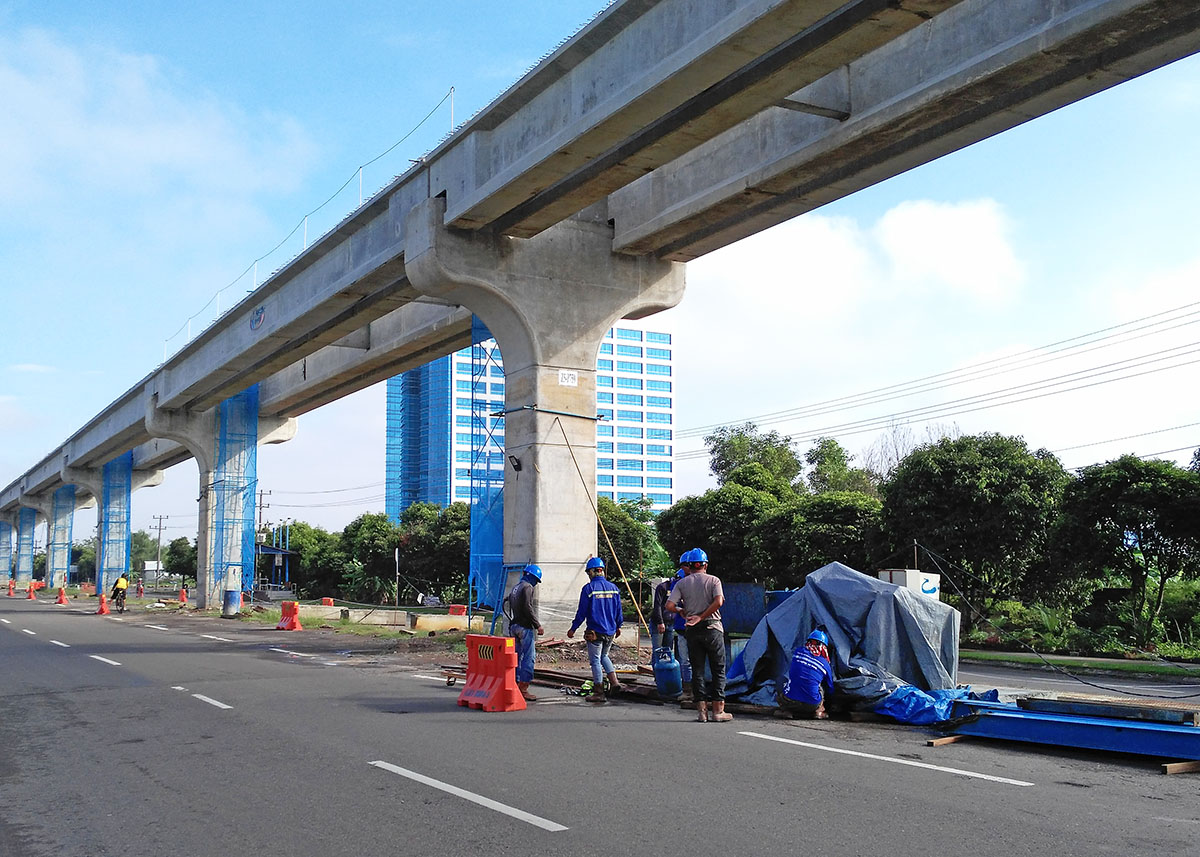
\includegraphics[scale=0.2]{gambar/lrt.jpg}
    \caption{Pembangunan LRT Palembang (Todes/bulletinmetropolis.com, 2017)}
    \label{fig:lrt}
\end{figure}

Selain dampak dari segi pembangunan kota dampak lain dari kegiatan tersebut adalah meningkatnya jumlah wisatawan yang berkunjung ke Kota Palembang sehingga turut meningkatkan kepariwisataan Kota Palembang. Statistik kunjungan kota Palembang ditunjukkan ditunjukkan pada Gambar \ref{fig:bps}.\\

\begin{figure}[H]
  \centering
    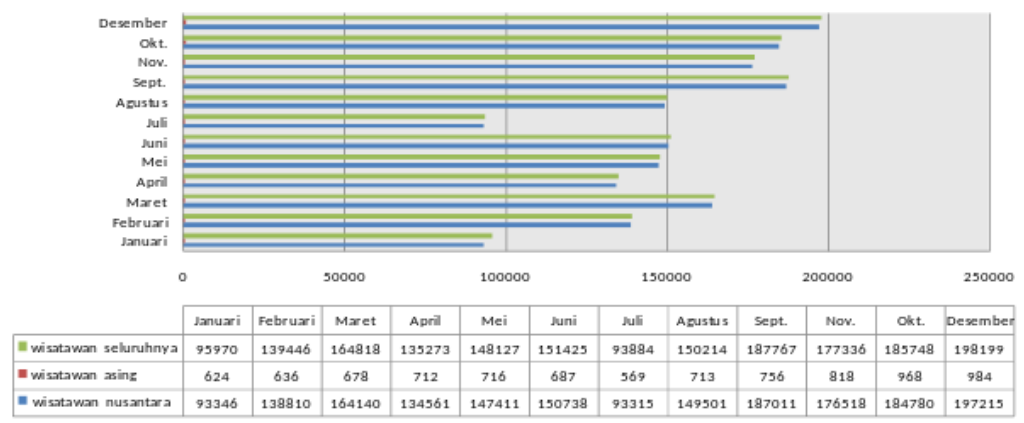
\includegraphics[scale=0.41]{gambar/bps.png}
    \caption{Statistik kunjungan wisata ke Kota Palembang (BPS Kota Palembang, 2014}
    \label{fig:bps}
\end{figure}

Berdasarkan Gambar \ref{fig:bps} terlihat bahwa terjadi peningkatan jumlah wisatawan yang masuk ke Palembang. Wisatawan lokal dan manca negara banyak berdatangan untuk menghadiri berbagai kegiatan yang diadakan di Palembang, hal ini ikut memicu banyaknya pemesanan hotel, penggunaan fasilitas umum berupa hotel, supermarket, pasar, halte bus, mesin ATM, rumah sakit, restoran atau rumah makan, tempat hiburan, tempat wisata dan lain sebagainya untuk mendukung kegiatan para wisatawan selama berada dan tinggal di Palembang.\

Untuk membantu mobilitas wisatawan yang datang ke Palembang maka dibutuhkan sebuah media yang dapat membantu mereka mendapatkan info mengenai event-event, sarana transportasi, serta fasilitas publik untuk mengakomodasi mereka selama event-event tersebut berlangsung. Informasi tersebut saat ini belum tersedia secara komprehensif bagi para wisatawan. Website-website resmi dari pemerintah hanya menampilkan informasi kegiatan serta berita-berita lain tentang Palembang, tetapi belum ada informasi yang cukup tentang fasilitas publik kota Palembang.\ 
Kota Palembang telah memiliki portal informasi resmi pada alamat http://www.palembang.go.id/. Terdapat informasi-informasi publik untuk berbagai bidang seperti kesehatan, pendidikan, pariwisata, dll.\
\begin{figure}[H]
  \centering
    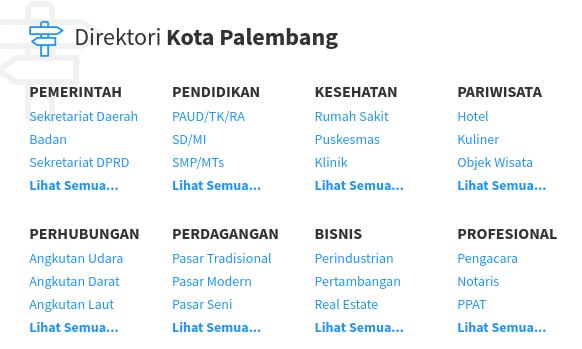
\includegraphics[scale=0.7]{gambar/palembanggoid.png}
    \caption{Potongan Website Direktori Kota Palembang (Pemerintah Kota Palembang, 2017)}
    \label{fig:plgportal}
\end{figure}
Pada gambar \ref{fig:plgportal} terdapat informasi-informasi mengenai kota Palembang yang terbagi kedalam direktori-direktori. Setiap informasi dipisahkan oleh \emph{link-link}  yang berbeda. Pengguna harus melakukan navigasi berulang kali untuk mendapatkan informasi-informasi yang berbeda tersebut. Cohen dalam Booth (2015) menyatakan bahwa sistem navigasi seperti ini (\emph{menu-based systems}) dapat digunakan untuk mencari informasi dengan mudah, tetapi kemampuan pencariannya sudah ditentukan sebelumnya dan tidak fleksibel.\

Oleh karena itu, untuk mengatasi keterbatasan tersebut dapat digunakan bahasa alami. Kauffman dalam Booth (2015) menyatakan bahwa bahasa alami lebih baik dalam menyatakan pertanyaan atau perintah, terlebih yang membutuhkan informasi negasi, jumlah dan informasi temporal. Bahasa alami juga mengurangi waktu penyelesaian suatu tugas.\

Penggunaan pencarian berbasis semantik pada sistem yang akan diajukan diharapkan dapat memberikan hasil yang lebih sesuai dengan konteks yang diinginkan pengguna. Penelitian tentang pencarian berbasis semantik pernah dilakukan oleh Admojo (2015), pada penelitian tersebut digunakan input dari query bahasa alami yang seterusnya akan ditulis \emph{NLP (Natural Language Processing)}. Domain Ontologi yang digunakan pada penelitian tersebut adalah \emph{linguistic} dan \emph{mountaineering}. Hasil penelitian mampu memahami input bahasa alami secara sintaksis dan secara semantik.\

Booth (2015) dalam penelitiannya mengembangkan sebuah bahasa query untuk perencanaan perjalanan yang diberi nama \emph{TRANQUYL}. Selanjutnya mereka juga mengembangkan software bernama \emph{NL2TRNQUYL} yang menerjemahkan input bahasa inggris menjadi \emph{query} yang dimengerti oleh \emph{TRANQUYL}. Sistem tersebut mampu mengerti \emph{request} dari user baik itu berupa kalimat utuh ataupun hanya potongan kalimat saja.\

Berdasarkan penelitian-penelitian tersebut diusulkan sebuah sistem dimana pengguna bisa memberikan input berupa \emph{query NLP} dalam bahasa Indonesia dan mendapatkan hasil sesuai dengan yang diharapkan.


\section{Rumusan Masalah}
Rumusan masalah dalam penelitian ini adalah bagaimana menyediakan informasi \emph{event} dan fasilitas publik Kota Palembang yang memadai bagi wisatawan  dengan input pengguna berupa bahasa alami.\


\section{Batasan Masalah}
Agar penelitian ini tetap fokus maka diberikan batasan-batasan sebagai berikut:
\begin{enumerate}
  \item Input bahasa yang digunakan menggunakan bahasa Indonesia
  \item Data fasilitas publik yang ditampilkan berupa Rumah Sakit, Tempat Ibadah, Tempat Wisata dan Tempat Makan
  \item Data koordinat fasilitas publik didapat dari layanan \emph{Foursquare} dan \emph{Google Map API}.
  \item Bahasa Pemrograman yang akan digunakan pada thesis ini adalah \emph{PHP} untuk \emph{Backend}, \emph{Javascript} pada bagian \emph{Frontend}. \emph{Database} menggunakan \emph{RDF Triple Store}, yang akan di akses menggunakan sebuah \emph{project Open Source} bernama \emph{Apache Jena Fuseki}.
  \item Sistem akan memberikan \emph{output} berupa \emph{JSON} yang dapat di konsumsi oleh \emph{client} lintas platform. 
\end{enumerate}


\section{Tujuan Penelitian}
Tujuan dari penelitian ini adalah menghasilkan piranti lunak yang memberikan solusi untuk permasalahan pencarian informasi kegiatan beserta fasilitas publik kota Palembang dengan menyusun ontologi untuk merepresentasikan basis pengetahuan berupa data fasilitas umum di Kota Palembang beserta rute transportasinya berdasarkan input \emph{NLP}.


\section{Manfaat Penelitian}
Manfaat dari penelitian ini adalah:
\begin{enumerate}
  \item Membantu wisatawan mendapatkan informasi publik fasilitas umum di Kota Palembang.
  \item Membantu wisatawan mendapatkan informasi kegiatan-kegiatan di Kota Palembang.
\end{enumerate}

\section{Sistematika Penulisan}
\noindent
\textbf{BAB I : PENDAHULUAN}

Pada bab ini dijelaskan latar belakang, rumusan masalah, batasan, tujuan, manfaat, dan sistematika penulisan.\\

\noindent
\textbf{BAB II : TINJAUAN PUSTAKA}

Pada bab ini diuraikan teori-teori dasar yang berkaitan dengan penelitian-penelitian yang telah dilakukan.\\

\noindent
\textbf{BAB III : LANDASAN TEORI}

Pada bab ini dijelaskan teori-teori dasar yang berkaitan dengan penelitian yang dilakukan dan akanmenjadi dasar dalam pemecahan masalah.\\

\noindent
\textbf{BAB IV : ANALISIS DAN RANCANGAN SISTEM}

Pada bab ini dijelaskan perancangan ontologi bahasa dan fasilitas publik Kota Palembang, proses pada setiap tahapan pada rancangan arsitektur penelitian serta perancangan antarmuka sistem.\\

\noindent
\textbf{BAB V : IMPLEMENTASI}

Bab ini berisikan pembuatan class, property, dan instance pada ontologi yang digunakan serta pembahasan proses yang terjadi dari input \emph{NLP} pengguna sampai ke hasil akhir yang dapat diproses oleh antarmuka sistem.\\

\noindent
\textbf{BAB V : HASIL DAN PEMBAHASAN}

Pada bab ini dijelaskan hasil penelitian dan pembahasannya.\\

\noindent
\textbf{BAB V : KESIMPULAN DAN SARAN}

Pada bab ini ditulis kesimpulan akhir dari penelitian dan saran untuk pengembangan penelitian selanjutnya.\\

% Baris ini digunakan untuk membantu dalam melakukan sitasi
% Karena diapit dengan comment, maka baris ini akan diabaikan
% oleh compiler LaTeX.
\begin{comment}
\bibliography{daftar-pustaka}
\end{comment}


%!TEX root = ./template-skripsi.tex
%-------------------------------------------------------------------------------
%                            BAB II
%               TINJAUAN PUSTAKA DAN DASAR TEORI
%-------------------------------------------------------------------------------

\chapter{TINJAUAN PUSTAKA DAN DASAR TEORI}                

\section{Tinjauan Pustaka}
  Lorem ipsum is a pseudo-Latin text used in web design, typography, layout, and printing in place of English to emphasise design elements over content. It's also called placeholder (or filler) text. It's a convenient tool for mock-ups. It helps to outline the visual elements of a document or presentation, eg typography, font, or layout. Lorem ipsum is mostly a part of a Latin text by the classical author and philospher Cicero. Its words and letters have been changed by addition or removal, so to deliberately render its content nonsensical; it's not genuine, correct, or comprehensible Latin anymore. While lorem ipsum's still resembles classical Latin, it actually has no meaning whatsoever. As Cicero's text doesn't contain the letters K, W, or Z, alien to latin, these, and others are often inserted randomly to mimic the typographic appearence of European languages, as are digraphs not to be found in the original. \cite{DaSilvaCampos2011}

\section{Landasan Teori}
  \subsection{\LaTeX}
    Ne per tota mollis suscipit. Ullum labitur vim ut, ea dicit eleifend dissentias sit. Duis praesent expetenda ne sed. Sit et labitur albucius elaboraret. Ceteros efficiantur mei ad. Hendrerit vulputate democritum est at, quem veniam ne has, mea te malis ignota volumus.

    Eros reprimique vim no. Alii legendos volutpat in sed, sit enim nemore labores no. No odio decore causae has. Vim te falli libris neglegentur, eam in tempor delectus dignissim, nam hinc dictas an.

    Pro omnium incorrupte ea. Elitr eirmod ei qui, ex partem causae disputationi nec. Amet dicant no vis, eum modo omnes quaeque ad, antiopam evertitur reprehendunt pro ut. Nulla inermis est ne. Choro insolens mel ne, eos labitur nusquam eu, nec deserunt reformidans ut. His etiam copiosae principes te, sit brute atqui definiebas id.


      \begin{figure}[H]
        \centering
          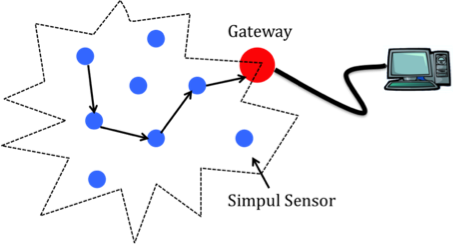
\includegraphics{gambar/wsn}
          \caption{Jaringan sensor nirkabel.}
          \label{wsn}
      \end{figure}


  \subsection{Sublime Text}
    Et affert civibus has. Has ne facer accumsan argumentum, apeirian hendrerit persequeris pro ex. Suscipit vivendum sensibus mea at, vim ei hinc numquam, at dicit timeam dissentiet mel. At patrioque intellegebat sea, error argumentum dissentias sea in.

    Quo no atqui omnesque intellegat, ne nominavi argumentum quo. Eum ei purto oporteat dissentiet, soleat utamur an sit. Et assum dicam interpretaris quo. Cetero alterum ea vel, no possit alterum utroque nec. His fuisset quaestio ad. Has eu tritani incorrupte consequuntur, esse aliquip nec ne.

% Baris ini digunakan untuk membantu dalam melakukan sitasi
% Karena diapit dengan comment, maka baris ini akan diabaikan
% oleh compiler LaTeX.
\begin{comment}
\bibliography{daftar-pustaka}
\end{comment}


%!TEX root = ./thesis-main.tex
%-------------------------------------------------------------------------------
%                            BAB III
%               		     LANDASAN TEORI
%-------------------------------------------------------------------------------

\chapter{LANDASAN TEORI}

\section{Web Semantik}
	Alat dan bahan yang digunakan pada penelitian ini terbagi atas perangkat keras dan perangkat lunak yang akan dijelaskan seperti berikut.

\section{\emph{Resource Description Framework (RDF)}}
	Menurut \emph{W3C} RDF adalah sebuah model standar pertukaran data di Web. RDF mampu menggabungkan data walaupun skema  yang mendasari berbeda, dan secara khusus mendukung evolusi skema dari waktu ke waktu tanpa memerlukan semua konsumen data diubah.

	RDF secara umum dinyatakan menggunakan sesuatu yang dikenal sebagai \emph{triple} yang merupakan unit dasar dari sebuah informasi. Sebuah \emph{triple} terdiri dari \emph{subject}, \emph{predicate} dan \emph{object}.

	Sebuah contoh sederhana dari dokumen RDF ditunjukkan pada gambar \ref{fig:rdfinstance}

	\begin{figure}[H]
		\centering
			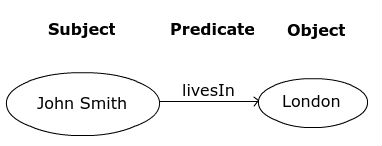
\includegraphics[scale=0.65]{gambar/rdfinstance.jpg}
			\caption{Sebuah representasi RDF untuk sebuah informasi}
			\label{fig:rdfinstance}
	\end{figure}

	Ide sederhana dari unit informasi ini adalah bahwa unit informasi tersebut dapat dinyatakan dalam berbagai format yang dengan mudah di mengerti oleh mesin. \emph{RDFS (RDF Schema)} digunakan untuk menggambarkan properti dan kelas dari sebuah dokumen \emph{RDF}. Pewujudan dari triple pada gambar \ref{fig:rdfinstance} dapat dinyatakan dalam XML dan JSON berikut:

	\begin{figure}[H]
		\centering
			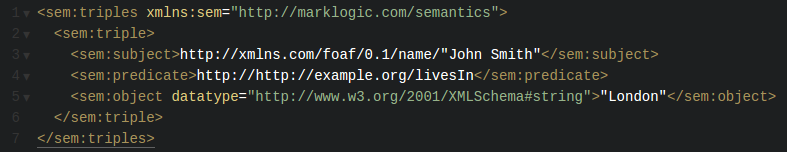
\includegraphics[scale=0.5]{gambar/rdfinstancexml.png}
			\caption{RDF dalam format XML}
			\label{fig:rdfinstancexml}
	\end{figure}

	\begin{figure}[H]
		\centering
			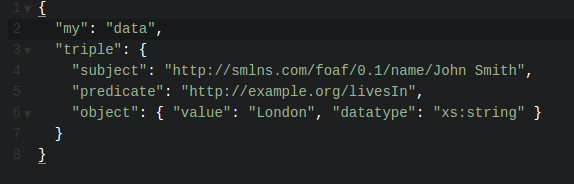
\includegraphics[scale=0.5]{gambar/rdfinstancejson.png}
			\caption{RDF dalam format JSON}
			\label{fig:rdfinstancejson}
	\end{figure}

\section{\emph{Web Ontology Language (OWL)}}
	\emph{Web Ontology Language (OWL)} atau Ontologi adalah sebuah standar dari \emph{W3C} untuk membantu perkembangan Web Semantik. \emph{OWL} memberikan interpretasi mesin yang lebih besar dengan memberikan kosa kata tambahan beserta semantik lainnya. \emph{OWL} menambahkan lebih banyak kosakata untuk menggambarkan \emph{RDFS (RDF Schema)}. Konsep ini merupakan ide dasar dibalik peningkatan kemampuan mesin untuk dapat mengerti dengan menggunakan \emph{OWL}

	\emph{OWL} dikategorikan menjadi tiga sub bahasa agar sesuai dengan kebutuhan pengguna: 

	\vspace{-0.5cm}

	\begin{enumerate}[a.]
	\begin{singlespace}
	\itemsep0em
		\item \emph{OWL DL} -- \emph{DL} merupakan singkatan dari \emph{Description Logics}, yang merupakan salah satu bidang dasar untuk penciptaan \emph{OWL}. \emph{OWL DL} diperuntukkan bagi pengguna yang ingin mencapai ekspresivitas penuh suatu topik sambil memastikan bahwa perhitungan akan selesai pada waktu yang terbatas,
		\item \emph{OWL Lite} -- Sebuah sub bahasa sederhana yang menyediakan hirarki dan batasan klasifikasi. Kardinalitas hanya bisa memiliki nilai 0 atau 1, sehingga membatasi dan mengurangi kompleksitas hubungan,
		\item \emph{OWL Full} -- \emph{OWL Full} ditujukan untuk pengguna yang perlu melintasi seluruh hierarki subjek ke akarnya dan bahkan \emph{metadata} dari \emph{root}. \emph{OWL Full} tidak memiliki jaminan komputasi karena cukup dapat dimengerti bahwa proses ini bisa sangat kompleks. Namun, \emph{OWL Full} mendorong untuk menciptakan semua kemungkinan makna kelas \emph{RDF}.
	\end{singlespace}
	\end{enumerate}

\section{Ontologi}
Ontologi tidak memiliki definisi yang diterima secara formal. Namun, kosakata dan ontologi sering digunakan dengan makna yang sama. Ontologi dapat didefinisikan sebagai seperangkat \emph{URI} yang membentuk makna untuk topik tertentu. Unit yang membentuk ontologi adalah satu set \emph{RDF} bersama dengan \emph{OWL}. Ada berbagai ontologi yang telah diciptakan dan sering digunakan. Namun sebagian besar ontologi diciptakan oleh manusia dan mesin memiliki sedikit sekali kontribusi dalam hal ini.

Contoh beberapa ontologi: \emph{Dublin Core} -- Mereka memiliki ontologi untuk metadata data. Kumpulan ontologi mereka mencakup kelas, properti, skema pengkodean kosa kata, skema pengkodean sintaks dan koleksi. Semua dari mereka memiliki beberapa set \emph{RDF} yang menjelaskan data tentangnya. \emph{Dbpedia} - "Ini adalah upaya bersama komunitas untuk mengambil informasi terstruktur dari \emph{Wikipedia} dan membuat informasi ini tersedia di Web. \emph{Dbpedia} memungkinkan Anda untuk mengajukan pertanyaan yang canggih terhadap Wikipedia, dan untuk menghubungkan kumpulan data yang berbeda pada data Web ke Wikipedia. Lebih jauh lagi, dbpedia mungkin mengilhami mekanisme baru untuk navigasi, kaitan, dan peningkatan ensiklopedia itu sendiri." Kutipan di atas adalah deskripsi resmi \emph{Dbpedia} dari pembuatnya. Bisa dikatakan bahwa \emph{Dbpedia} adalah versi Web Semantik dari \emph{Wikipedia}. Ontologi \emph{Dbpedia} sangat besar dan memiliki 4,2 juta objek yang mencakup hal-hal, orang, tempat, pekerjaan, organisasi, dan spesies. Jumlah data yang besar ini disusun menggunakan \emph{RDF} dan \emph{OWL}. Beberapa di antaranya terkait dengan sumber data terkait lainnya yang mengubah Dbpedia menjadi inti dari jaringan data seperti yang telah disebutkan.

Ada berbagai contoh ontologi seperti \emph{FOAF}, \emph{Good Relations}, \emph{Music Ontology} dll. Sekarang semua ontologi ini perlu disimpan di suatu tempat dan untuk tujuan itu kita memiliki \emph{Triple Stores}.

\section{\emph{Triple Stores}}
\emph{Triple Store} adalah jenis khusus \emph{database} untuk menyimpan dan mengambil \emph{triples}. \emph{Triple stores} dibuat khusus untuk \emph{Semantic Web} dan \emph{Linked Data}. Serupa dengan \emph{database} yang lain \emph{triple store} mengambil informasi melalui bahasa \emph{query}. \emph{Triple Store} juga memiliki kemampuan untuk mengimpor dan mengekspor informasi yang dibutuhkan dalam format \emph{RDF}.

Ada banyak varian yang berbeda dari Triple Stores, beberapa di antaranya diciptakan dari nol dan beberapa di antaranya dibangun di atas database \emph{SQL} dan \emph{NoSQL} yang telah ada. \emph{Triple Store} sering juga disebut sebagai \emph{RDF Store}. Beberapa contoh \emph{Triple Stores} adalah:

\begin{enumerate}[a.]
	\item \emph{Virtuoso} -- adalah middleware yang mendukung Sistem Manajemen Database Relasi Tradisional (RDBMS) dan juga memiliki dukungan khusus untuk penyimpanan dan pengambilan dokumen \emph{RDF}. \emph{Virtuoso} mendukung beberapa protokol dan menggunakan proses \emph{multi-threaded} tunggal. Hal ini juga dikenal sebagai \emph{Openlink Virtuoso}. Virtuoso menyediakan \emph{SPARQL Endpoint} seperti semua \emph{Triple Store} lainnya. \emph{Virtuoso} terkenal dengan kinerjanya dalam mengolah \emph{dataset} besar. Misalnya, \emph{Dbpedia} di-host di \emph{Virtuoso Triple Store}.
	\item \emph{Fuseki} -- adalah proyek turunan dari \emph{Apache Jena}. \emph{Fuseki} menyediakan server \emph{RDF} yang bisa menjadi \emph{Triple Store}, yang dapat dikelola melalui protokol \emph{REST}. \emph{Fuseki} bisa berjalan sebagai service pada mesin remote, \emph{WAR (Java Web Archieve)} atau sebagai \emph{server standalone}. \emph{Fuseki} mendukung \emph{SPARQL 1.1} dan juga menambahkan dukungan logging untuk memantau apa yang terjadi di \emph{triple store}. Versi terbaru \emph{Fuseki v2}, memberikan fitur keamanan melalui \emph{Apache Shiro}. \emph{Apache Shiro} menambahkan kriptografi dan manajemen sesi ke \emph{Fuseki}. 
\end{enumerate}

\section{\emph{SPARQL}}
\emph{SPARQL} adalah standar \emph{W3C} lain dalam kategori \emph{Semantic Web}. \emph{SPARQL} adalah bahasa query yang mirip dengan \emph{Structured Query Language (SQL)} untuk \emph{Relational Database Management Systems (RDBMS)}. \emph{SPARQL} digunakan untuk melakukan \emph{query} dokumen \emph{RDF}. Hal ini memungkinkan representasi grafik dari dokumen \emph{RDF}. \emph{Query SPARQL} bisa menghasilkan set grafik. Hasilnya bisa berupa nilai literal ataupun \emph{URI}. Kemampuan untuk mengambil literal atau bahkan mengubah \emph{URI} menjadi label memberikan cara langsung dan mudah bagi aplikasi untuk menggunakan hasil \emph{query}.

\section{Jadwal Kegiatan}

	% Please remember to add \use{multirow} to your document preamble in order to suppor multirow cells
		\begin{table}[H]
		\centering
		\caption{Jadwal Penelitian.}
		\label{jadwal}
		\begin{tabular}{|c|l|l|l|l|l|l|l|}
		\hline
		\multirow{2}{*}{No} & \multirow{2}{*}{Keterangan} & \multicolumn{6}{c|}{Bulan}                                                                                                                          \\ \cline{3-8} 
		                    &                             & 1 & 2 & 3 & 4 & 5 & 6 \\ \hline
		1                   & Studi literatur                                  &\cellcolor{gray} &\cellcolor{gray}&                        &                        &                        &                         \\ \hline
		2                   & Desain                                           &                        &\cellcolor{gray}&\cellcolor{gray}&                        &                        &                         \\ \hline
		3                   & Pembelian bahan                                  &                        &                        &\cellcolor{gray}&                        &                        &                         \\ \hline
		4                   & Pembuatan prototipe                              &                        &                        &\cellcolor{gray}&\cellcolor{gray}&\cellcolor{gray}&                         \\ \hline
		5                   & Uji coba dan perbaikan                           &                        &                        &                        &\cellcolor{gray}&\cellcolor{gray}&                         \\ \hline
		6                   & Penulisan skripsi                                &                        &                        &                        &                        &                        &\cellcolor{gray}\\ \hline
		\end{tabular}
		\end{table}
	
% Baris ini digunakan untuk membantu dalam melakukan sitasi
% Karena diapit dengan comment, maka baris ini akan diabaikan
% oleh compiler LaTeX.
\begin{comment}
\bibliography{daftar-pustaka}
\end{comment}


%!TEX root = ./thesis-main.tex
%-------------------------------------------------------------------------------
%                            BAB IV
%         		ANALISIS DAN RANCANGAN SISTEM
%-------------------------------------------------------------------------------

\chapter{ANALISIS DAN RANCANGAN SISTEM}
	\section{Gambaran Umum Sistem}
	Penelitian ini ditujukan untuk memberikan informasi tentang Kota Palembang berdasarkan input \emph{NLP} dari pengguna. Sistem menerima input berupa \emph{query} bahasa alami dalam bahasa Indonesia. Sistem memproses input untuk dipahami dan hasilnya digunakan untuk melakukan pencarian informasi. Hasil pencarian informasi kemudian disajikan kepada pengguna.

	Data informasi fasilitas publik kota Palembang didapatkan dari \emph{Foursquare API} serta \emph{Google API} dalam format \emph{JSON}. Data tersebut akan diubah kedalam format \emph{RDF} agar dapat di akses menggunakan \emph{SPARQL Query}.Setiap tahapan proses yang dikerjakan sistem menggunakan basis pengetahuan yang direpresentasikan ke dalam 2 ontologi, yaitu ontologi Bahasa untuk merepresentasikan pengetahuan dibidang linguistik dan ontologi Informasi Publik Kota Palembang. Ontologi bahasa yang akan digunakan menggunakan ontologi yang telah dibuat sebelumnya oleh Admojo (2015) dan kemudian di tambahkan kosakata baru berkaitan informasi publik kota Palembang dikarenakan kosakata pada ontologi tersebut ditujukan untuk domain pendakian.
	
	Beberapa input yang dapat diproses dalam penelitian ini:
	\begin{enumerate}[a.]
		\item Carikan Hotel dalam radius 2 km dari Bandara
		\item Lokasi GOR Jakabaring Palembang
		\item Tampilkan daftar Event pada tanggal 16 November 2017
	\end{enumerate}
	
	Setelah input diterima akan dilakukan proses \emph{tokenizing}. Kata-kata yang telah di-\emph{tokenize} akan diubah menjadi bentuk kata baku, serta diperiksa \emph{spelling} dari setiap kata tersebut dengan membandingkan dengan data yang ada pada ontologi bahasa. Pada tahapan berikutnya, kata-kata tersebut akan diklasifikasikan ke dalam kelas-kelas seperti \emph{Event}, \emph{StopPoint}, \emph{ReligiousPlaces}, \emph{Shops}, dsb. Berdasarkan hasil kategori yang didapat kemudian dibuat \emph{query SPARQL} ke ontologi Informasi Publik Kota Palembang sehingga dihasilkan informasi yang dibutuhkan.
	
	\section{Desain Sistem}
	Sistem yang dikembangkan pada penelitian ini merupakan sistem berbasis web. Pengguna dapat melakukan pencarian informasi fasilitas publik kota Palembang  menggunakan web browser dengan input berupa bahasa alami yaitu bahasa Indonesia. Untuk memproses input hingga menghasilkan informasi, sistem terbagi menjadi dua komponen yaitu: \emph{Query Preprocessing} dan \emph{Query Mapping}. 
	
	Secara umum tahapan kerja sistem yang diusulkan ditunjukkan pada Gambar \ref{fig:arsitektur}.
	
	\begin{figure}[H]
		\centering
		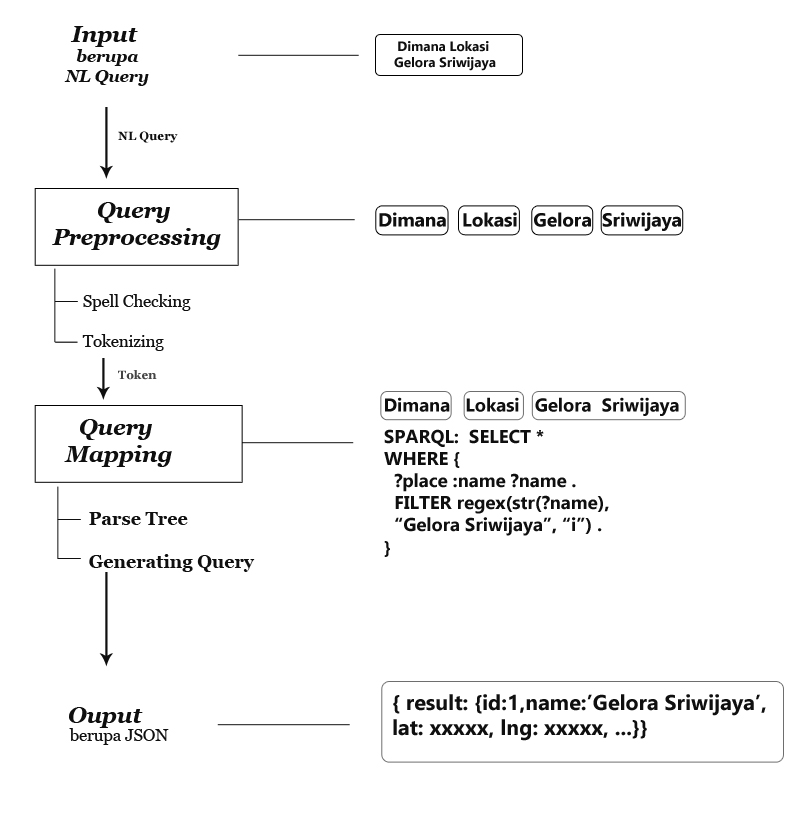
\includegraphics[scale=0.50]{gambar/arsitektur.png}
		\caption{Ilustrasi tahapan kerja sistem yang diusulkan}
		\label{fig:arsitektur}
	\end{figure}
	
	
	\subsection{\emph{Query Preprocessing}}
	Pada tahap \emph{Query Preprocessing} dilakukan validasi dan pengubahan input menjadi urutan kata (\emph{token}). Proses validasi dilakukan dengan memeriksa setiap kata input dengan kata yang terdapat dalam ontologi (ontologi Bahasa dan ontologi Informasi Publik Kota Palembang). Input dinyatakan valid apabila setiap token ada didalam ontologi. 
	
	Satuan kata pada urutan kata dapat mengandung satu kata atau lebih. Misalnya pada kata "Gelora" dan "Sriwijaya" seperti yang diilustrasikan pada Gambar \ref{fig:querypreprocessing}, berdasarkan pengetahuan pada ontologi Informasi Fasilitas Publik Kota Palembang, kata "Gelora Sriwijaya" merupakan nama untuk sebuah stadion yang berada di Kota Palembang. Oleh karena itu, sistem membakukan kata "Gelora" dan "Sriwijaya" menjadi "Gelora Sriwijaya".
	
	Proses pembentukan input menjadi urutan kata juga melibatkan pengambilan atribut tiap kata dari ontologi (ontologi Bahasa). Atribut tersebut yaitu Atribut Sintaksis yang digunakan untuk proses pengecekan sintaksis serta atribut semantik. 
	
	\begin{figure}[H]
		\centering
		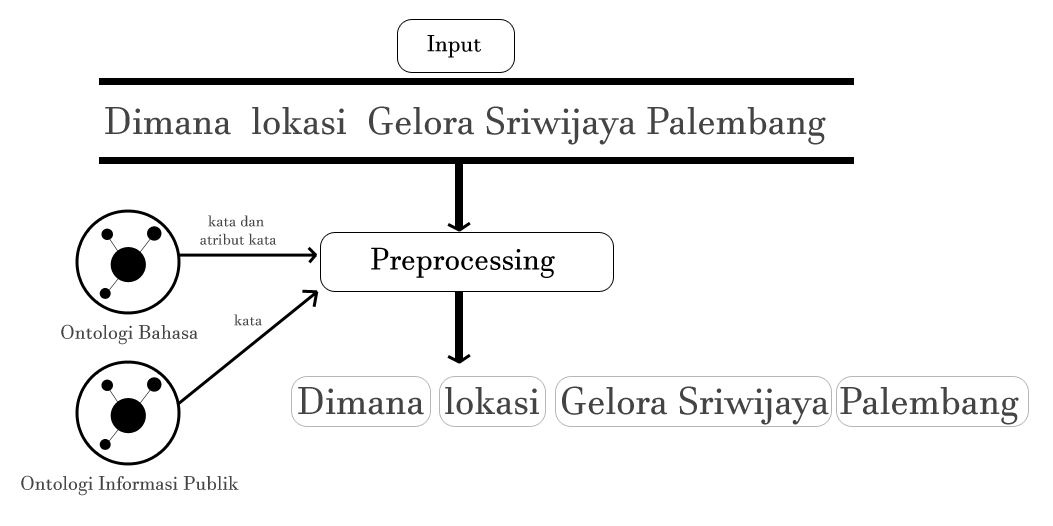
\includegraphics[scale=0.50]{gambar/querypreprocessing.png}
		\caption{Ilustrasi tahapan kerja sistem yang diusulkan}
		\label{fig:querypreprocessing}
	\end{figure}
	
	\subsection{\emph{Query Mapping}}
	Pada tahapan ini urutan \emph{token} yang didapatkan pada tahapan \emph{query preprocessing} di bentuk menjadi sebuah \emph{parse tree} dengan mencocokkan atribut sintaksis serta atribut semantik dari setiap \emph{token} menggunakan aturan-aturan tata bahasa Indonesia. Hasil dari \emph{parse tree} tersebut akan digunakan sebagai dasar pembentukan \emph{query SPARQL}. \emph{Query} dijalankan pada ontologi informasi publik kota Palembang sehingga menghasilkan jawaban dari \emph{query} yang diinput. Hasil jawaban dibentuk menggunakan format \emph{JSON} sehingga dapat di proses oleh \emph{client lintas platform}.
	
	Gambar \ref{fig:parsetree} menggambarkan pembentukan \emph{parse tree}.
	
	\begin{figure}[H]
		\centering
		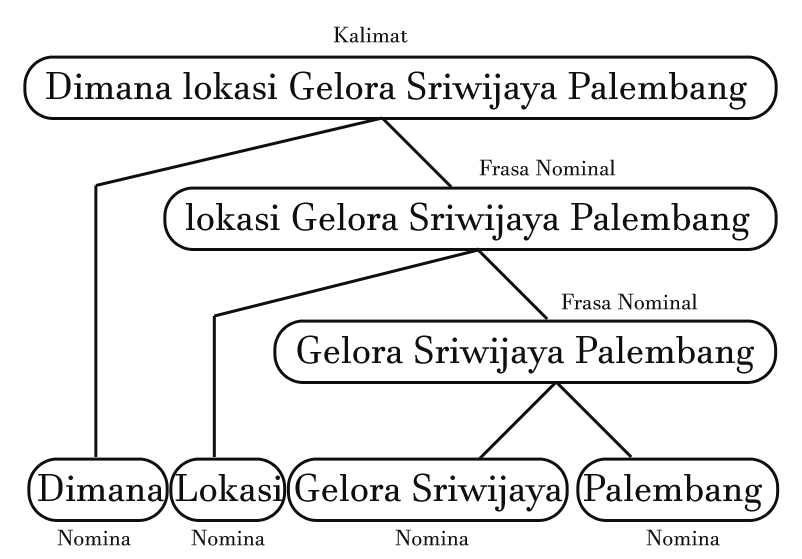
\includegraphics[scale=0.45]{gambar/parsetree.png}
		\caption{Ilustrasi pembentukan Parse Tree}
		\label{fig:parsetree}
	\end{figure}
	
	\section{Perancangan Ontologi}
	
	\subsection{Ontologi Bahasa}
	Pengetahuan bahasa yang digunakan dalam penelitian ini berkaitan dengan pengetahuan bidang linguistik yakni meliputi pengetahuan tentang kata, hubungan kata, kategori kata, fungsi sintaksis, dan perilaku semantik dari satuan bahasa. Pengetahuan sintaksis dan pengetahuan semantik digunakan pada proses pemahaman input menggunakan tata bahasa Indonesia baku yang dikemukakan oleh Alwi dkk., (2003).
	
	Pengetahuan sintaksis dan pengetahuan semantik dinyatakan dalam aturan-aturan gramatikal yang direpresentasikan menggunakan \emph{Unification Based Grammar} berdasarkan formalisme penulisan gramatikal yang telah dikemukakan oleh (Suryawan, 2013; Gazdar dan Mellish, 1989). 
	
	Pengetahuan pada ontologi Bahasa dideskripsikan ke dalam konsep konsep yang disusun berdasarkan suatu klasifikasi dan dikelompokkan ke dalam \emph{class-class} yang sama. Konsep yang digunakan pada ontologi Bahasa didasarkan pada konsep bahasa yang telah dideskripsikan oleh Suryawan (2013), yang dikembangkan sesuai dengan kebutuhan sistem pada penelitian ini.
	
	Pada penelitian ini digunakan ontologi bahasa yang telah dibuat sebelumnya pada penelitian Admojo (2013). Ontologi tersebut dikembangkan dengan menambahkan kata-kata baru yang berkaitan dengan informasi publik kota Palembang. Ontologi sebelumnya difokuskan pada kata-kata yang berkaitan dengan istilah-istilah \emph{mountaineering} sehingga perlu ditambahkan kosa kata baru yang dibutuhkan pada penelitian ini.
	
	Class yang dibentuk dalam ontologi Bahasa yaitu \emph{Lexicon}, \emph{WordCategory}, \emph{Semantic}, \emph{SemanticType}, \emph{QueryLogic}. Setiap class berada dalam domain yang sama, namun menyimpan konsep pengetahuan yang berbeda-beda. Hirarki antar class dideskripsikan pada Gambar \ref{fig:classontologibahasa}.
	
	\begin{figure}[H]
		\centering
		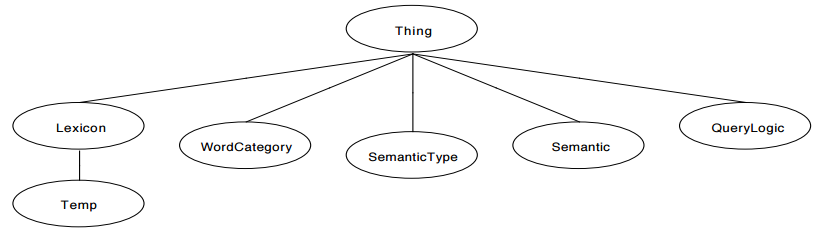
\includegraphics[scale=0.45]{gambar/classontologibahasa.png}
		\caption{\emph{Class-class} pada ontologi bahasa}
		\label{fig:classontologibahasa}
	\end{figure}
	
	Class Lexicon adalah representasi dari konsep kata yang merupakan satuan bahasa terkecil. Setiap individual yang terdapat di dalam class \emph{Lexicon} memiliki kategori, peran dan fungsi di dalam kalimat yang dideskripsikan menggunakan property, yaitu: \emph{word, category, semanticValue, type, argCat0, argCat1, argCat2, stripCat, argType0, argType1, argType2, stripType}. \emph{Property} yang digunakan untuk mendeskripsikan kata dijabarkan pada tabel 3.
	
	// tabel lagi disini
	
	Properti yang dijabarkan pada Tabel 3 memiliki fungsi, yaitu: Properti \emph{word} digunakan untuk mendeskripsikan struktur lahir suatu kata. Properti \emph{category} digunakan untuk mendeskripsikan kategori sintaksis yang dimiliki kata. Properti \emph{type} digunakan untuk mendeskripsikan tipe semantik yang dimiliki kata. Properti \emph{semanticValue} digunakan untuk mendeskripsikan nilai semantik kata Properti \emph{argCat0, argCat1, argCat2} dan \emph{stripCat} digunakan untuk mendeskripsikan hubungan perilaku sintaksis suatu kata, frasa, klausa, kalimat. Properti \emph{argType0, argType1, argType2} dan \emph{stripType} digunakan untuk mendeskripsikan hubungan perilaku semantik suatu kata, frasa, klausa, kalimat.
	
	\emph{Class SemanticType} merupakan realisasi dari konsep tentang perilaku semantik yang dimiliki oleh suatu kata. Konsep tentang perilaku semantik tidak dideskripsikan dengan menggunakan properti apapun.
	
	\emph{Class Semantic} merupakan realisasi dari konsep tentang nilai semantik dari suatu kata atau suatu satuan bahasa. Konsep tentang nilai semantik dari suatu kata atau suatu satuan bahasa tidak dideskripsikan dengan menggunakan properti apapun.
	
	\emph{Class WordCategory} merupakan realisasi dari konsep tentang kategori sintaksis. Konsep tentang kategori sintaksis tidak dideskripsikan dengan menggunakan properti apapun.
	
	\emph{Class QueryLogic} merupakan realisasi dari konsep informasi semantik dari suatu satuan bahasa. Konsep tentang makna dari suatu satuan bahasa dideskripsikan dengan menggunakan dua buah properti, yaitu: \emph{parA} dan \emph{qpart}. 
	
	\subsection{Ontologi Informasi Publik Kota Palembang}
	Ontologi informasi publik kota Palembang merupakan representasi dari pengetahuan tentang hal-hal yang dapat dicari oleh pengguna melalui sistem ini. Pengetahuan tersebut meliputi \emph{event-event} baik nasional maupun internasional yang diadakan di Palembang serta beberapa \emph{Point of Interest} yang meliputi tempat makan, tempat-tempat keagamaan, penginapan, toko, serta \emph{stop point} seperti halte \emph{busway}, halte \emph{LRT}, dsb. Gambar \ref{fig:classhierarchy} merupakan \emph{Class Hierarchy} yang akan digunakan pada sistem yang diusulkan.
	
	\begin{figure}[H]
		\centering
		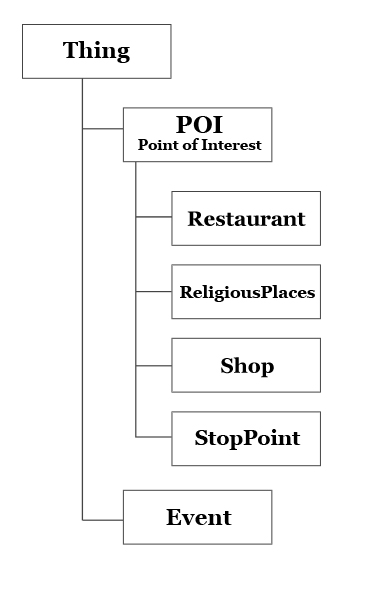
\includegraphics[scale=0.45]{gambar/classhierarchy.png}
		\caption{Struktur \emph{class hierarchy} sistem yang diusulkan}
		\label{fig:classhierarchy}
	\end{figure}
	
	Tabel menggambarkan properti minimum untuk mendeskripsikan konsep \emph{Point of Interest}
	
	

	\section{Perancangan Antarmuka}
		Habeo perfecto in sea. Ea deleniti gloriatur pri, paulo mediocrem incorrupte sea ei. Ad mollis scripta per. Incorrupte sadipscing ne mel. Mel ex nonumy malorum epicurei.

		Ne per tota mollis suscipit. Ullum labitur vim ut, ea dicit eleifend dissentias sit. Duis praesent expetenda ne sed. Sit et labitur albucius elaboraret. Ceteros efficiantur mei ad. Hendrerit vulputate democritum est at, quem veniam ne has, mea te malis ignota volumus.

		Eros reprimique vim no. Alii legendos volutpat in sed, sit enim nemore labores no. No odio decore causae has. Vim te falli libris neglegentur, eam in tempor delectus dignissim, nam hinc dictas an.
	
	\section{Subbab 2}		
		Habeo perfecto in sea. Ea deleniti gloriatur pri, paulo mediocrem incorrupte sea ei. Ad mollis scripta per. Incorrupte sadipscing ne mel. Mel ex nonumy malorum epicurei.

		\subsection{Subsubbab 2 1}
			Ne per tota mollis suscipit. Ullum labitur vim ut, ea dicit eleifend dissentias sit. Duis praesent expetenda ne sed. Sit et labitur albucius elaboraret. Ceteros efficiantur mei ad. Hendrerit vulputate democritum est at, quem veniam ne has, mea te malis ignota volumus.
			
			\begingroup
			    \fontsize{10pt}{12pt}\selectfont
			    \begin{verbatim}
					config mount
				        option target        /mnt
				        option device        /dev/sda1
				        option fstype        ext3
				        option options       rw,sync
				        option enabled       1
				        option enabled_fsck  0
				        option is_rootfs     1
			    \end{verbatim}  
			\endgroup

			\begingroup
			    \fontsize{10pt}{12pt}\selectfont
			    \begin{verbatim}
					# opkg update
					# opkg install python pyserial
			    \end{verbatim}  
			\endgroup			

		\subsection{Subsubbab 2 2}
			Consul graeco signiferumque qui id, usu eu summo dicunt voluptatum, nec ne simul perpetua posidonium. Eos ea saepe prodesset signiferumque. No dolore possit est. Mei no justo intellegebat definitiones, vis ferri lorem eripuit ad. Solum tritani scribentur duo ei, his an adipisci intellegat.

	\section{Subab 3}
		Consul graeco signiferumque qui id, usu eu summo dicunt voluptatum, nec ne simul perpetua posidonium. Eos ea saepe prodesset signiferumque. No dolore possit est. Mei no justo intellegebat definitiones, vis ferri lorem eripuit ad. Solum tritani scribentur duo ei, his an adipisci intellegat.
			
			
% Baris ini digunakan untuk membantu dalam melakukan sitasi.
% Karena diapit dengan comment, maka baris ini akan diabaikan
% oleh compiler LaTeX.
\begin{comment}
\bibliography{daftar-pustaka}
\end{comment}

%!TEX root = ./template-skripsi.tex
%-------------------------------------------------------------------------------
%                            	BAB V
%               		KESIMPULAN DAN SARAN
%-------------------------------------------------------------------------------

\chapter{KESIMPULAN DAN SARAN}

\section{Kesimpulan}
	Berdasarkan hasil analisis dan pengujian fungsional aplikasi ini, didapat kesimpulan sebagai berikut:

	\begin{enumerate}
		\item Lorem ipsum is a pseudo-Latin text used in web design, typography, layout, and printing in place of English to emphasise design elements over content. 
		
		\item It's also called placeholder (or filler) text. It's a convenient tool for mock-ups. 
		
		\item It helps to outline the visual elements of a document or presentation, eg typography, font, or layout. Lorem ipsum is mostly a part of a Latin text by the classical author and philospher Cicero.

		\item Its words and letters have been changed by addition or removal, so to deliberately render its content nonsensical; it's not genuine, correct, or comprehensible Latin anymore. 
	\end{enumerate}


\section{Saran}
	\begin{enumerate}
		\item Lorem ipsum is a pseudo-Latin text used in web design, typography, layout, and printing in place of English to emphasise design elements over content. 
		
		\item It's also called placeholder (or filler) text. It's a convenient tool for mock-ups. 
		
		\item It helps to outline the visual elements of a document or presentation, eg typography, font, or layout. Lorem ipsum is mostly a part of a Latin text by the classical author and philospher Cicero.

		\item Its words and letters have been changed by addition or removal, so to deliberately render its content nonsensical; it's not genuine, correct, or comprehensible Latin anymore. 
	\end{enumerate}

	
% Baris ini digunakan untuk membantu dalam melakukan sitasi
% Karena diapit dengan comment, maka baris ini akan diabaikan
% oleh compiler LaTeX.
\begin{comment}
\bibliography{daftar-pustaka}
\end{comment}


%-----------------------------------------------------------------
%Disini akhir masukan Bab
%-----------------------------------------------------------------


%-----------------------------------------------------------------
% Disini awal masukan untuk Daftar Pustaka
% - Daftar pustaka diambil dari file .bib yang ada pada folder ini
%   juga.
% - Untuk memudahkan dalam memanajemen dan menggenerate file .bib
%   gunakan reference manager seperti Mendeley, Zotero, EndNote,
%   dll.
%-----------------------------------------------------------------
\bibliography{IEEEabrv,daftar-pustaka}
\addcontentsline{toc}{chapter}{DAFTAR PUSTAKA}
%-----------------------------------------------------------------
%Disini akhir masukan Daftar Pustaka
%-----------------------------------------------------------------

\end{document}